\documentclass[pdftex,12pt,a4paper]{article}

\usepackage{graphicx}  
\usepackage[margin=2.5cm]{geometry}
\usepackage{breakcites}
\usepackage{indentfirst}
\usepackage{pgfgantt}
\usepackage{pdflscape}
\usepackage{float}
\usepackage{epsfig}
\usepackage{epstopdf}
\usepackage[cmex10]{amsmath}
\usepackage{stfloats}
\usepackage{multirow}

\renewcommand{\refname}{REFERENCES}
\linespread{1.3}

\usepackage{mathtools}
%\newcommand{\HRule}{\rule{\linewidth}{0.5mm}}
\thispagestyle{empty}
\begin{document}
\begin{titlepage}
\begin{center}
\textbf{}\\
\textbf{\Large{ISTANBUL TECHNICAL UNIVERSITY}}\\
\vspace{0.5cm}
\textbf{\Large{COMPUTER ENGINEERING DEPARTMENT}}\\
\vspace{2cm}
\textbf{\Large{BLG 242E\\ DIGITAL CIRCUITS LABORATORY\\ EXPERIMENT REPORT}}\\
\vspace{2.8cm}
\begin{table}[ht]
\centering
\Large{
\begin{tabular}{lcl}
\textbf{EXPERIMENT NO}  & : & 9 \\
\textbf{EXPERIMENT DATE}  & : & 19.04.2019 \\
\textbf{LAB SESSION}  & : & FRIDAY - 14.00 \\
\textbf{GROUP NO}  & : & G13 \\
\end{tabular}}
\end{table}
\vspace{1cm}
\textbf{\Large{GROUP MEMBERS:}}\\
\begin{table}[ht]
\centering
\Large{
\begin{tabular}{rcl}
{
150180704  & : & C\.{I}HAT AKK\.{I}RAZ \\
150180707  & : & FAT\.{I}H ALTINPINAR \\
150180734  & : & S\.{I}NAN \c{S}AR \\
}
\end{tabular}}
\end{table}
\vspace{2.8cm}
\textbf{\Large{SPRING 2019}}

\end{center}

\end{titlepage}

\newpage

\thispagestyle{empty}
\centering{\LARGE{ \textbf{ETHIC FORM}}}\\
\centering{\LARGE{\textbf{for}}}\\
\centering{\LARGE{\textbf{BLG242E Logic Circuits Laboratory}}}\\[0.2cm]
As a student of \\Istanbul Technical University Faculty of Computer and Informatics Engineering;
\begin{enumerate}
    \item I will not attempt to cheat in quizes and final exam,
    \item I will not use disallowed sources or tools (mobile phone, calculator etc.) during the exam,
    \item I will not write any information (formula, text, figure etc.) on the table, sheets or books that are allowed to be used during the exam,
    \item I will give reference when using printed or online published sources,
    \item I will not use the results in a source as they are, or by changing a part of them without giving a reference,
    \item I will not show unused sources as used, 
    \item I will not present someone else’s idea as my own idea, 
    \item I will not make someone do my homework, project or thesis for money or anything else,
    \item I will not take an exam or enter a lecture on behalf of others,
    \item I will not make excuses for not attending in exams or lessons by taking reports from someone I know (medical doctor parents or relatives),
    \item I will refrain from deliberately harming the public materials at our university,  
    \item I will comply with the safety rules in laboratory work,
    \item I will behave in accordance with the rules of respect for the lecturers and teaching assistants
\end{enumerate}
\vspace{-1em}
\centering{\LARGE{signed by}}\\
\vspace{-1em}
\begin{table}[ht]
\centering
\begin{tabular}{rcl}
150180704  & : & C\.{I}HAT AKK\.{I}RAZ \\
150180707  & : & FAT\.{I}H ALTINPINAR \\
150180734  & : & S\.{I}NAN \c{S}AR \\
\end{tabular}
\end{table}
\vspace{-1em}
 \begin{table}[ht]
 \begin{tabular}{lr}
%\textbf{Date:\hspace*{1.0cm}/\hspace*{1.0cm}/} &\qquad \qquad\qquad\qquad \qquad\qquad\qquad \qquad\qquad\qquad \qquad\qquad \textbf{SIGNED}\\
\end{tabular}
\end{table} % adds the ethic sign
\addcontentsline{toc}{section}{\numberline {}ETHICS}
\newpage

\thispagestyle{empty}
\addtocontents{toc}{\contentsline {section}{\numberline {}FRONT COVER}{}}
\addtocontents{toc}{\contentsline {section}{\numberline {}CONTENTS}{}}
\setcounter{tocdepth}{4}
\tableofcontents
\clearpage

\setcounter{page}{1}

\section{INTRODUCTION}

In this experiment, 1-bit ALU is designed and implemented, then capability of this 1-bit ALU is extended to 4-bit ALU using serial approach.

\section{REQUIREMENTS}
\begin{flushleft}
\underline{Tools Used}\cite{booklet}
\end{flushleft}
\begin{itemize}
    \item C.A.D.E.T
    \item 74000 series ICs
    \begin{itemize}
        \item 74xx08 - Quadruple 2-input Positive AND Gates
        \item 74xx32 - Quadruple 2-input Positive OR Gates
        \item 74xx83 - 4-bit Binary Full Adder
        \item 74xx86 - Quadruple 2-input Positive Exclusive Or (XOR) Gates
        \item 74xx151 - 8:1 Multiplexer
        \item 74xx174 - Hex D-Type Flip-Flops
        
    \end{itemize}
\end{itemize}

\begin{flushleft}
\subsection{PART 1}

\paragraph{}
In the first part of the experiment, 1-bit ALU is designed and implemented using necessary logic gates as given in the figure below. Logic switches are used as input(A,B,$C_{in}$) and outputs are observed via LEDs.

\begin{figure}[h]
	\centering
	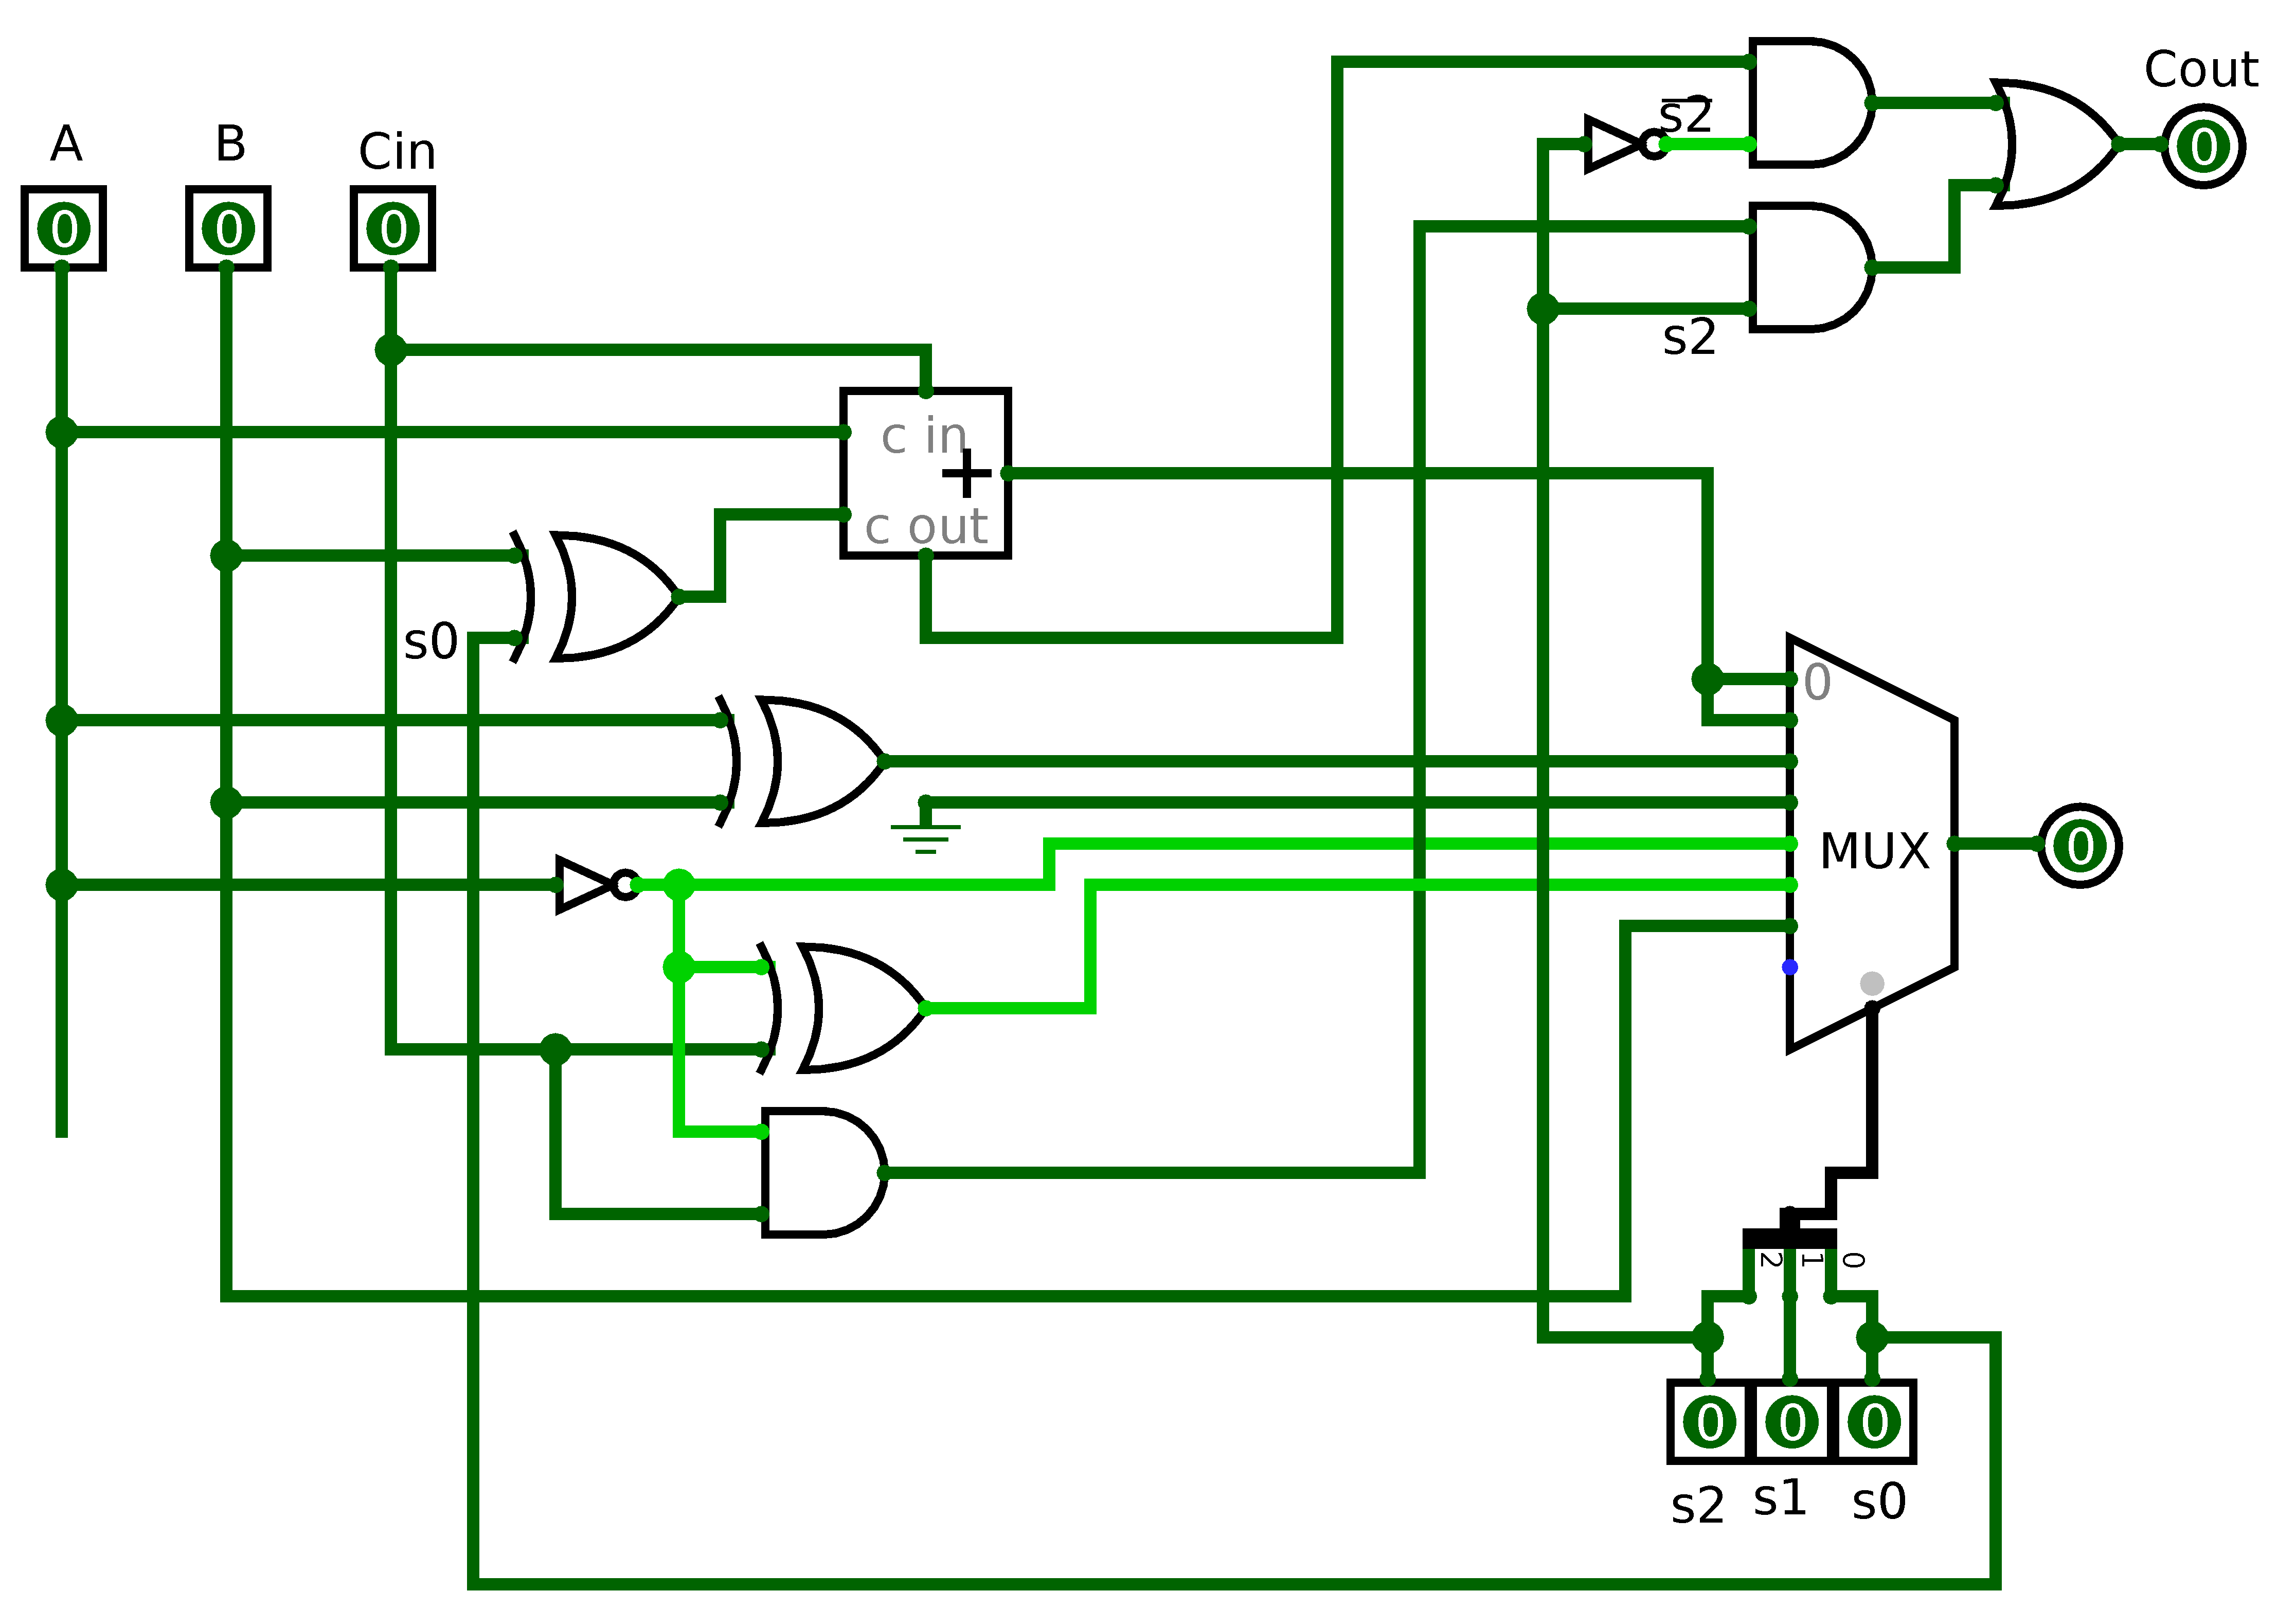
\includegraphics[width=0.7\textwidth]{ALU.png}	
	\caption{1-bit ALU Circuit}
	\label{circ:part1}
\end{figure}

\paragraph{}
This 1-bit ALU is performing 7 different operations below.

\begin{table}[h]
    \centering
    \begin{tabular}{c|c}
        Operations & RTL  \\ \hline
        Addition with Carry & $C_{out}O\leftarrow$ A + B + $C_{in}$ \\
        Subtraction & $C_{out}O\leftarrow$ A + B' + $C_{in}$ \\
        XOR & $O\leftarrow$ A $\oplus$ B  \\
        Clear & $O\leftarrow$ 0 \\
        Complement & $O\leftarrow$ A' \\
        Two Complement & $O\leftarrow$ A' + $C_{in}$ \\
        Transfer B & $O\leftarrow$ B\\
    \end{tabular}
    \caption{1-bit ALU Operations}
    \label{1bitaluoperations}
\end{table}

\paragraph{}
After this implementation, tests are performed for given cases above. Observed outputs are validated with calculations before the experiment. 

%Test Cases

\begin{table}[]
    \centering
    \begin{tabular}{c|c|c|c|c|c}
         Selector & A & B & $C_{in}$ & $C_{out}$ & Output  \\ \hline
         000 & 1 & 1 & 1 & 1 & 0 \\   
         001 & 1 & 1 & 1 & 1 & 0 \\   
         010 & 1 & 0 & - & - & 1 \\  
         011 & 0 & 1 & - & - & 0 \\
         
         100 & 0 & - & - & - & 1 \\   
         101 & 1 & - & 1 & - & 0 \\ 
         110 & - & 1 & - & - & 1 \\
    \end{tabular}
    \caption{Test Cases for 1-bit ALU}
    \label{tab:my_label}
\end{table}

\subsection{PART 2}
\paragraph{}
In the final part of the experiment, capabilities of 1-bit ALU are extended to 4-bit variables by using memory units. 4-bit ALU is implemented by using 1-bit ALU which is implemented in the previous part of the experiment. Using additional ALUs connected in parallel dramatically increases the complexity of the circuit. In this part, serial approach is used to overcome this challenge. 4-bit ALU is created via using a 1-bit ALU and memory units as shown given figure below.

\begin{figure}[h]
	\centering
	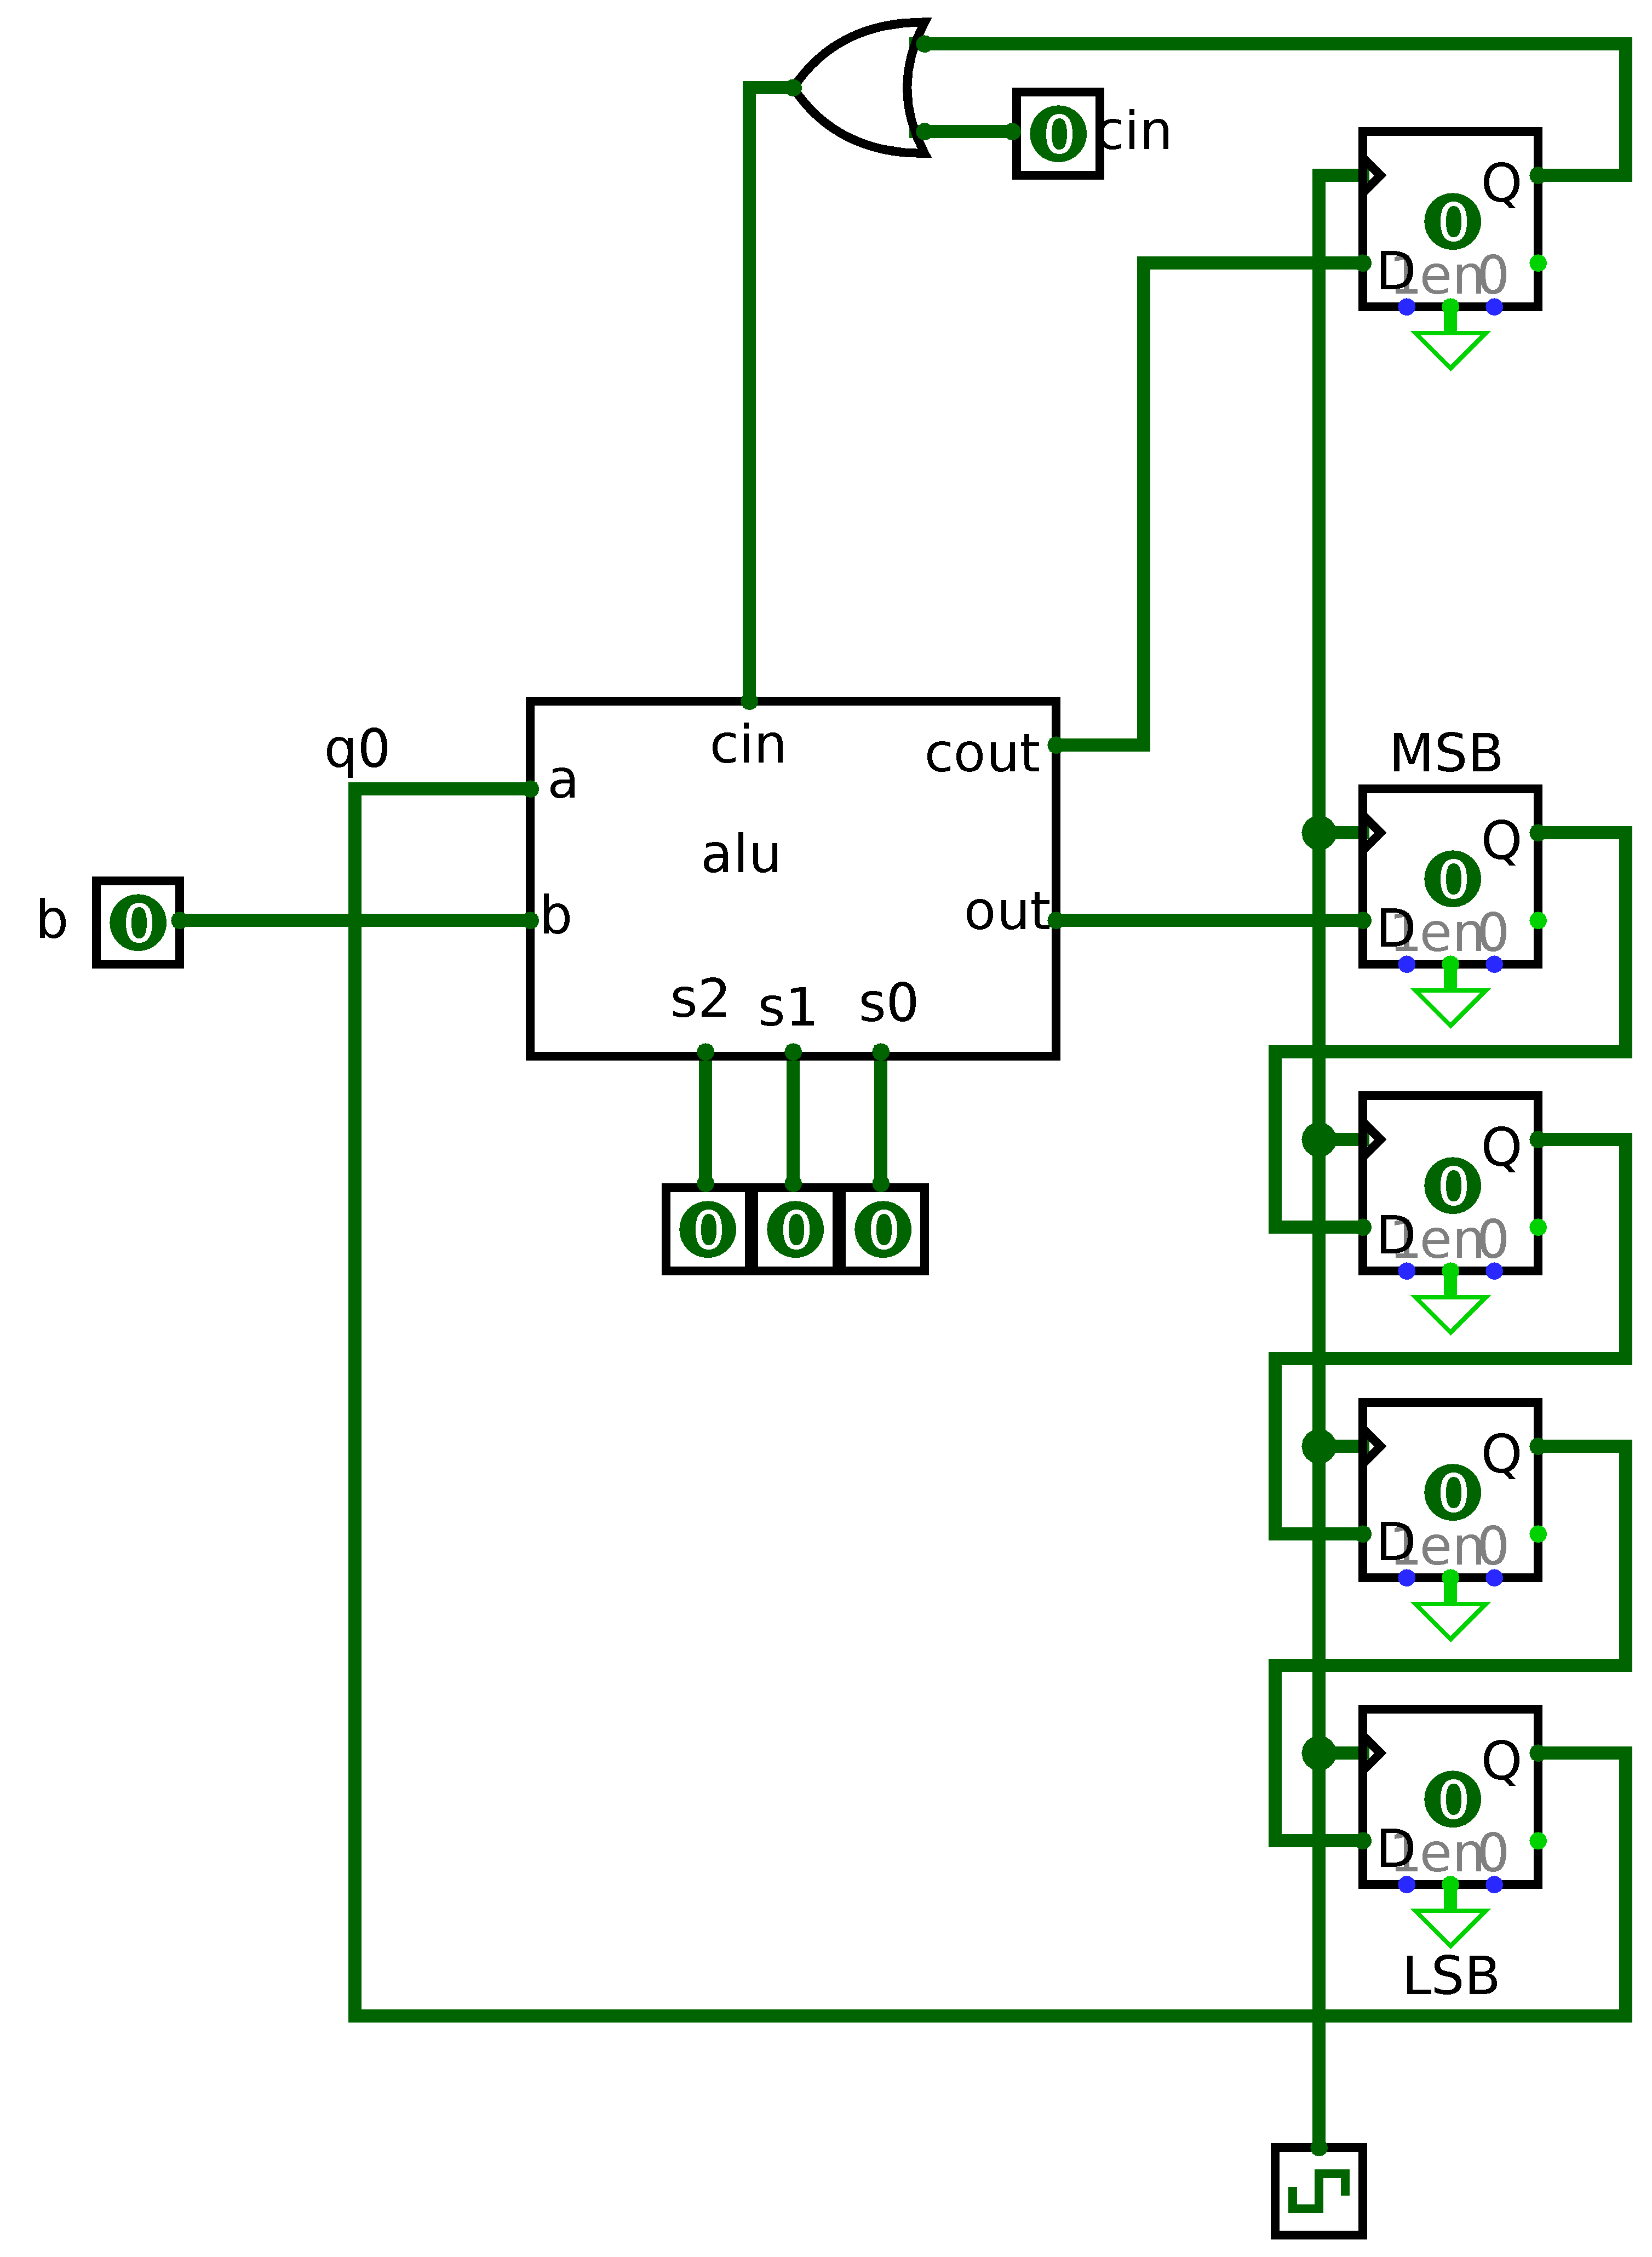
\includegraphics[width=0.7\textwidth]{4b.png}	
	\caption{4 Bit ALU using 1-bit ALUs}
	\label{circ:part2}
\end{figure}

\paragraph{}
 To do 4-bit operations on a 1-bit ALU, 4 clock cycles are required. This is achieved by applying least significant bit of the operand to B and applying least significant memory unit to A then the result is written to most significant memory unit every clock cycle. At the same time memory units are shifted from most significant towards least significant. Thus after the $4^{th}$ cycle, result of the operation that is applied on least significant bit is stored in least significant memory unit. $C_{in}$ is connected to $C_{out}$ which allows carry transferring between bits when required. User can also write $C_{in}$ and it should be only applied while doing an operation over least significant bit.

%Test Cases
\begin{table}[]
    \centering
    \begin{tabular}{c|c|c|c|c|c}
         Selector & A & B & $C_{in}$ & $C_{out}$ & Output  \\ \hline
         000 & 0010 & 1001 & 1 & 0 & 1100 \\   
         001 & 0101 & 0111 & 1 & 0 & 1110 \\   
         010 & 1010 & 0010 & - & - & 1000 \\  
         011 & 1110 & 0101 & - & - & 0000 \\
         100 & 0111 & - & - & - & 1000 \\  
         101 & 1100 & - & 1 & - & 
         0100 \\
         110 & - & 1011 & - & - & 1011 \\
    \end{tabular}
    \caption{Test Cases for circuit}
    \label{tab:my_label}
\end{table}



\end{flushleft}


\newpage
\section{INTERPRETATION OF THE RESULTS}
We were able to get consistent results throughout the both parts of the experiment (Details of both designs are given in the sections above.). The 1-bit ALU we designed worked without any issues. (However, display units on the CADET were causing some trouble while we were observing the results. After trying a few different LED's, we found some that worked without any issues.) Our extended 4-bit design also functioned flawlessly and was consistent with its implementation in Logisim.

\section{CONCLUSION}
The experiment taught us a different implementation technique to build an ALU with multiple bits. It decreases the complexity of the circuit but requires more clock cycles than a parallel approach. We also organised our actions in this experiment better than any previous experiments. Which led to faster and more reliable progress.

\newpage
\addcontentsline{toc}{section}{\numberline {}REFERENCES}

\bibliographystyle{unsrt}
\bibliography{reference}

\end{document}

